\chapter{Timing Diagram generator}
The 8085 Microprocessor is designed to execute 74 different types of instruction. Each instruction has two parts: OPCODE (operation code) and OPERAND. Each functions are divided into machine cycles and each cycles is further divided into T-states.

Basically, the microprocessor external communication functions can be divided into 3 categories of Machine Cycle:
\begin{enumerate}
\item Memory Read and Write
\item I/O Read and Write
\item Request Acknowledge
\end{enumerate}

Of which Request Acknowledge machine cycle is not yet supported in this version of the software, but internally it is simulated.
\\
There are three methods of Timing Diagram Generation :
\begin{enumerate}
\item Static Timing Diagram Generation
\item Dynamic Timing Diagram Generation
\begin{enumerate}
\item By Manual Step by Step Simulation
\item By Automatic Step by Step Simulation
\end{enumerate}
\end{enumerate}
\pagebreak
\section{Static Timing Diagram Generation}
To open the Timing Diagram window click the filled rows of the column named "T-states" in the Assembler workspace, as shown in \cref{fig:tstate:before:editor}. Static Timing Diagram is basically the machine cycles of the instruction in pre-simulation state. As, can be seen in \cref{fig:tstate:before:diagram} where default values(00H in this case) are loaded during the Memory Read Cycle of "LDA 1234H" from address 1234H.  
\begin{figure}[htbp]
\centering
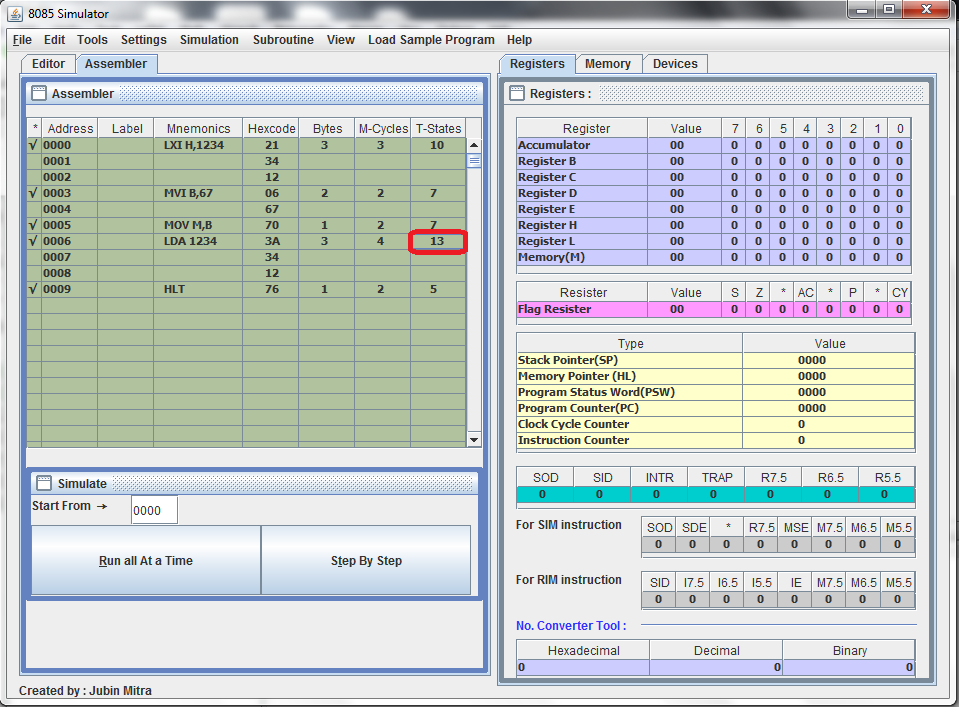
\includegraphics[width=0.75\linewidth]{./TStateEditorBefore}
\caption{The Red box marks the area of the Assembler workspace to be clicked before execution of the program}
\label{fig:tstate:before:editor}
\end{figure}
\begin{figure}[htbp]
\centering
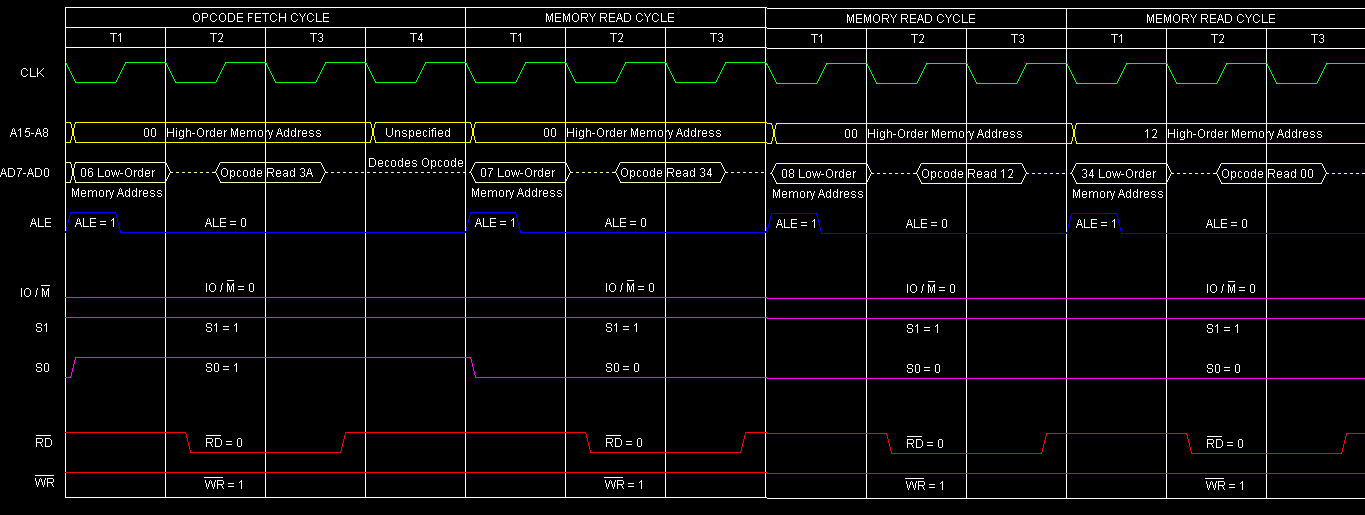
\includegraphics[width=\linewidth]{./TStateBefore}
\caption{Timing Diagram of "LDA 1234", where the last MEMORY READ CYCLE shows the value at address 1234H is set with default value 00H}
\label{fig:tstate:before:diagram}
\end{figure}
\pagebreak
\section{Dynamic Timing Diagram Generation By Manual Step by Step Simulation}
Dynamic Timing Diagram is the machine cycles of the instruction in real time simulation state. The stepping to the next instruction is controlled manually by the user, using "Step by Step" mode of execution. Here again as shown in \cref{fig:tstate:after:editor}, need to click on the column named "T-states" of the currently highlighted row. Note carefully in \cref{fig:tstate:after:diagram} that the values(67H in this case) are loaded in the Memory Read Cycle of "LDA 1234H" during reading of memory content at address 1234H. 

\begin{figure}[htbp]
\centering
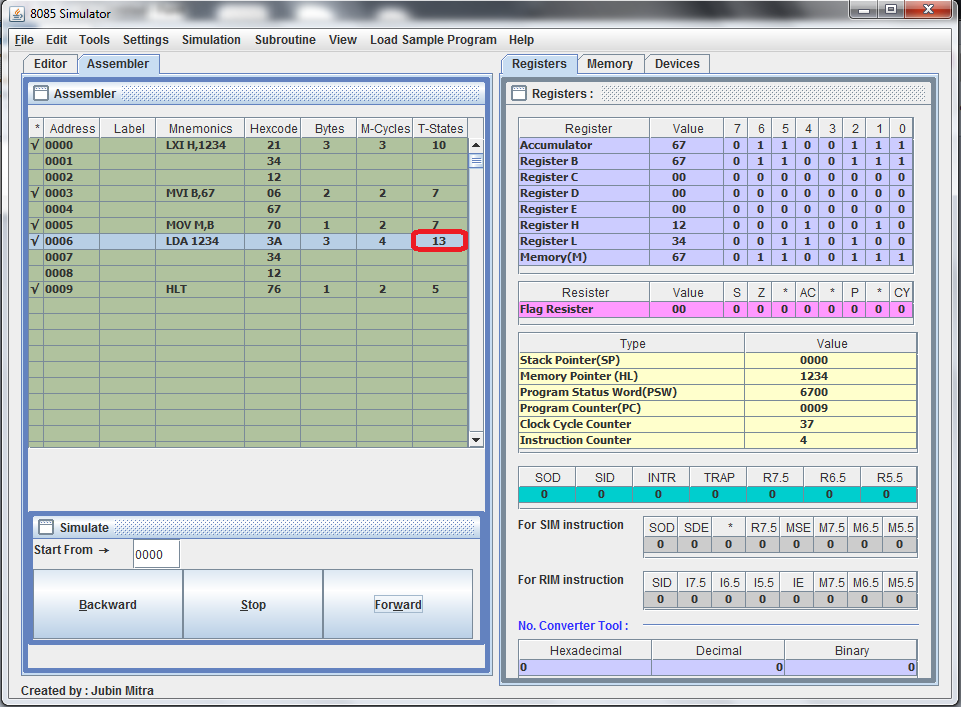
\includegraphics[width=0.75\linewidth]{./TStateEditorAfter}
\caption{The Red box marks the area of the Assembler workspace to be clicked during manual step by step simulation}
\label{fig:tstate:after:editor}
\end{figure}
\begin{figure}[htbp]
\centering
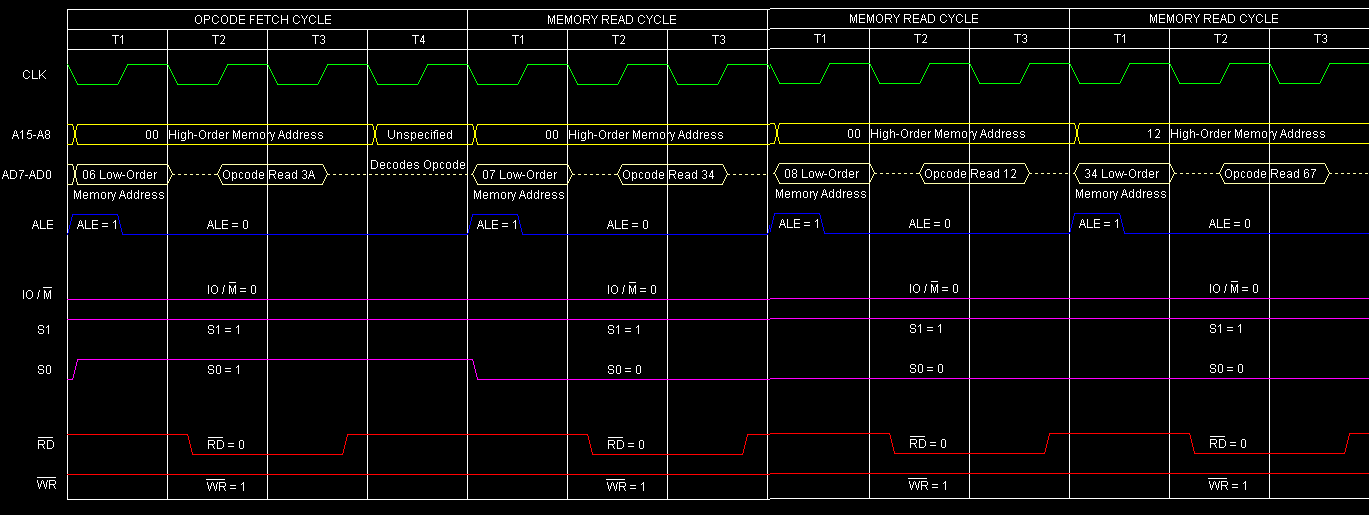
\includegraphics[width=\linewidth]{./TStateAfter}
\caption{Timing Diagram of "LDA 1234", where the last MEMORY READ CYCLE shows the value at address 1234H is loaded with 67H}
\label{fig:tstate:after:diagram}
\end{figure}
\pagebreak
\section{Dynamic Timing Diagram Generation By Automatic Step by Step Simulation}
Dynamic Timing Diagram is the machine cycles of the instruction in real time simulation state. The stepping to the next instruction is not controlled manually but by the simulator itself. As in this case user need to step down the "Run all at a Time" simulation speed to "Step by Step " mode of execution with user defined delay. Initially user need to open one time Static Timing Diagram Window, then it opens automatically and updates during each step of execution.